\section{问题一：基于拓扑结构的切图与任务调度}

\subsection{由独立分量到内部切分的决策}
场景 A 将子图边界转化为独立 Task 边界。第五章识别出的弱连通分量可以作为初始分配单位，在不切断内部依赖的条件下分散计算；单分量或负载高度集中的输入，则需要从内部切分获得并行机会。两类方案的取舍取决于新增并行工作量能否覆盖边界搬运和固定等待。

本问沿用式~\eqref{eq:q1-opgraph} 的操作依赖图和式~\eqref{eq:q1-features} 的双管道工作量。先以完整分量装箱得到低边界代价方案，再从分支、汇合及层宽变化构造少量替代划分；时间估计负责比较这些结构选择，局部任务重排与合并用于处理优先候选中的等待和冗余边界。

\subsection{场景 A 的约束与时间估计}
对给定核心数 $N\in\{2,3,4,5\}$，沿用子图映射 $\phi:O_c\to\mathcal S$，核心分配为 $a:\mathcal S\to\{0,\ldots,N-1\}$，核心 $k$ 的子图执行序列为 $\pi_k$。子图编号为非负整数；每个非 COPY 操作必须且只能分配到一个子图，每个子图必须且只能在一个核心序列中出现一次。子图依赖图以及加入同核先后关系后的联合图均须无环。输出采用附件规定的 \texttt{node\_to\_subgraph} 和 \texttt{core\_schedules} 两个字段。

以系统完工时间为主要优化目标，同时考虑新增 DDR 搬运量。根据固定配置，同核相邻 Task 的等待时间为 $\delta_{\rm same}=100$ cycle，跨核前驱 Task 的等待时间为 $\delta_{\rm cross}=1000$ cycle；各核心共同使用带宽 $\beta=60$ byte/cycle 的 DDR。L1 和 UB 的容量分别为 524288 byte 和 131072 byte。增加核心数不会增加 DDR 总带宽，同核 Task 切换也不能保留前一 Task 的缓存数据。

为在有限时间内比较候选，采用计算工作量、边界字节数和任务依赖共同构成时间估计。设 $I_s$、$U_s$ 为 Task $s$ 需要从 DDR 读入和写回 DDR 的张量集合，同一 Task 内按张量去重，则
\begin{equation}
\widehat B_A=\sum_{s\in\mathcal S}\left(\sum_{t\in I_s}s_t+\sum_{t\in U_s}s_t\right),\qquad
\widehat d_s=\max\left\{W_s^M,W_s^V,
\frac{\sum_{t\in I_s}s_t+\sum_{t\in U_s}s_t}{\beta}\right\}.
\label{eq:q1-duration}
\end{equation}
这里 $W_s^q$ 按式~\eqref{eq:q1-features} 对 Task 内操作重新求和。两条计算管道和搬运可以重叠执行，故采用三类工作量所需时间的最大值估计 Task 时长。$\widehat B_A$ 记录任务边界的读写量；缓存不足产生的换入换出尚未进入该估计，后续官方验收将保留这一部分实际开销。

在子图依赖图中加入同核相邻 Task 的顺序边，记得到的前驱集合为 $P^\pi(s)$。沿该图的拓扑序递推：
\begin{equation}
\begin{aligned}
\widehat f_s&=\widehat d_s+\max_{u\in P^\pi(s)}(\widehat f_u+\delta_{us}),\\
\widehat T_A&=\max\left\{\max_s\widehat f_s,\frac{\widehat B_A}{\beta}\right\},\qquad
\delta_{us}=\begin{cases}
\delta_{\rm cross},&a(u)\ne a(s),\\
\delta_{\rm same},&u\text{ 为 }s\text{ 的同核紧邻前项},\\
0,&\text{其余同核依赖}.
\end{cases}
\end{aligned}
\label{eq:q1-time}
\end{equation}
空前驱集合的最大值取 0。任务的预计启动时刻取决于前驱完成和同核队列的末端，两类约束在同一递推中合并。全局项 $\widehat B_A/\beta$ 则避免将共享 DDR 当作各核独享资源。该模型省略了逐个 COPY 请求的动态带宽竞争，适合对有限候选作快速排序；结果部分使用方案冻结后获得的官方完工时间与搬运量。

\subsection{分量装箱与结构切分}
首先将弱连通分量作为完整物品分配。按 $\max(W_j^M,W_j^V)$ 从大到小处理分量，设核心 $k$ 已分配的管道负载为 $(L_k^M,L_k^V)$，则将当前分量放入
\begin{equation}
k^*=\arg\min_k
\left(\max_{q\in\{M,V\}}(L_k^q+W_j^q),\ L_k^M+L_k^V,\ k\right).
\label{eq:q1-packing}
\end{equation}
括号内按字典序比较，选定后更新两条管道负载。同核分量合并为一个子图，空核保留空序列。该规则采用最长工作量优先分配思想\cite{Graham1969}，并用双管道负载替代单一处理时间。共享 DDR 和缓存使本题不再满足经典独立作业调度模型，因而不直接援引其近似比作为本算法的性能保证。

完整分配保留了每个分量内部的生产--消费关系，分量之间也没有计算依赖，因而能够减少中间张量的跨核搬运。共享输入仍可能被多个核心分别读取，核内空间不足仍会触发换入换出。若一个分量集中了大部分计算量，完整分配还会使负载集中在单核上。内部切分候选主要用于处理这一类并行度受限的输入。

内部切分围绕三类结构展开。第一类保留首次汇合前的独立分支，或按照末端消费者对分支归组；第二类利用拓扑层宽的收缩与扩张确定阶段边界；第三类按照深度带与源端、末端可达关系划分。在深度带构造中，候选边界附近按跨层张量字节数选择切分位置，以减少将大张量切到不同 Task 的情况。上述构造均保持原操作和依赖，不拆分操作，也不复制计算。

基础深度带宽由当前图的深度 $h$、总计算量 $W=\sum_{u\in O_c}c_u$ 和核心数确定：
\begin{equation}
w_0=\max\left\{2,\left\lceil\frac{N\delta_{\rm cross}h}{\max(1,W)}\right\rceil,
\left\lceil\frac{Nh}{256}\right\rceil\right\}.
\label{eq:q1-band}
\end{equation}
算法考察 $w_0,2w_0,4w_0$ 三种粒度。前一项避免过细切分，第二项使计算相对等待开销较小时倾向于更粗的 Task；第三项是固定的搜索规模控制规则，256 不是题目的硬件常数。此外，还保留减少活跃核心数的分量分配候选，以应对并行计算收益不足以抵消 DDR 争用的情形。

\subsection{任务列表调度与有限合并}
各结构候选先经过覆盖性、无环性检查和方案去重，再由式~\eqref{eq:q1-time} 排序。仅对排名靠前的至多三个候选进行任务调度与合并调整，以控制额外搜索量。

任务重排采用“就绪任务优先级--最早完成核心”的列表调度思想\cite{Topcuoglu2002}。先自后向前计算
\begin{equation}
r_s=\widehat d_s+\max_{v\in\operatorname{succ}(s)}(\delta_{\rm same}+r_v).
\label{eq:q1-rank}
\end{equation}
每次从全部已分配前驱的就绪 Task 中选取 $r_s$ 最大者，比较其放到各核心后的预计完成时刻。设 $F_k$ 是核心 $k$ 已排任务的末端时间，则
\begin{equation}
\operatorname{EFT}(s,k)=\widehat d_s+
\max\left\{F_k+\delta_{\rm same}\mathbf1[\pi_k\ne\varnothing],
\max_{u\in\operatorname{pred}(s)}
\big(\widehat f_u+\delta_{\rm cross}\mathbf1[a(u)\ne k]\big)\right\}.
\label{eq:q1-eft}
\end{equation}
优先选择 EFT 最小的核心，并列时依次选择已排 Task 数较少、编号较小的核心。式~\eqref{eq:q1-rank} 中的固定等待项只用于任务优先级；核心选择时则按式~\eqref{eq:q1-eft} 区分同核与跨核等待。这里采用尾部追加排布，没有执行 HEFT 的空闲区间插入步骤。

合并调整只考虑同核相邻、且在 Task 拓扑序中也相邻的任务对。每轮按共享张量字节数选取至多八对，分别计算收缩后的方案；联合依赖图有环的方案被剔除，在其余方案中选取能够降低 $\widehat T_A$ 的一项，最多执行两轮。任务重排与合并均从原结构候选独立出发，二者不串接。最终按预计时间、边界字节数和固定方案哈希依次比较；当完整分量方案与最优估计相差不超过 1\% 时，保留完整分量方案。该阈值降低了选择结果对微小估计误差的敏感性。

\begin{algorithmblock}{算法 6-1\quad 基于输入拓扑的切图与任务调度}
\alginput{当前计算图 $G$，核心数 $N$，带宽 $\beta$，等待参数 $\delta_{\rm same},\delta_{\rm cross}$。}
\algoutput{子图映射 $\phi$ 与每核子图序列 $\pi_0,\ldots,\pi_{N-1}$。}
\algline{读取张量、操作与边；提取非 COPY 操作集 $O_c$，保留原始数据。}
\algline{按生产--消费关系构建 $G_c$；计算拓扑序与节点深度 $d_u$。}
\algline{提取弱连通分量、层宽、分支及汇合位置，统计双管道工作量与张量字节数。}
\algline{按式~\eqref{eq:q1-packing} 构造完整分量方案 $P_0$，初始化待检验集合 $\mathcal B\leftarrow\{P_0\}$。}
\algline{将首次汇合、末端分支与较少活跃核心数的分量装箱候选加入 $\mathcal B$。}
\algline{按式~\eqref{eq:q1-band} 计算 $w_0$。}
\algline{\textbf{for} $w\in\{w_0,2w_0,4w_0\}$ \textbf{do}}
\algline[1]{构造数据感知深度带、分支汇合、层宽谷和末端可达归组候选，加入 $\mathcal B$。}
\algline{\textbf{end for}；将宽度为 $w_0$ 的源端可达归组候选加入 $\mathcal B$。}
\algline{逐项检验 $\mathcal B$，将覆盖完整、联合图无环且不重复的方案组成 $\mathcal P$；记录拒绝原因。}
\algline{按式~\eqref{eq:q1-duration}--\eqref{eq:q1-time} 评价 $\mathcal P$；按时间、字节数截取至多三个原始候选。}
\algline{\textbf{for} 所选方案中的每个 $P$ \textbf{do}}
\algline[1]{从 $P$ 分别生成就绪列表重排方案与至多两轮的相邻任务合并方案。}
\algline[1]{重新检查合法性，计算时间估计，将不同的合法方案加入 $\mathcal P$。}
\algline{\textbf{end for}}
\algline{取 $\widehat T_A$ 最小的 $P^*$；时间并列时比较边界字节数与固定方案哈希。}
\algline{若 $\widehat T_A(P_0)\le1.01\widehat T_A(P^*)$，令 $P^*\leftarrow P_0$。}
\algline{\textbf{return} $P^*$ 的 \texttt{node\_to\_subgraph} 与 \texttt{core\_schedules}。}
\end{algorithmblock}

\subsection{求解结果与分析}
算法对每个图、每种核数分别从原始输入生成方案。所有全局参数在正式运行前固定，生成过程中不读取历史方案和逐图得分，也不调用官方评估器。方案保存后，再使用未修改的附件程序完成 100 个图、2--5 核共 400 组验收，全部通过。

设第 $i$ 个图在 $N$ 核下的官方完工时间为 $T_{i,N}$，按题目规定采用的单核整图时间为 $T_{i,1}$。统计采用逐图加速比的算术平均：
\begin{equation}
S_{i,N}=\frac{T_{i,1}}{T_{i,N}},\qquad
\overline S_N=\frac1{100}\sum_{i=1}^{100}S_{i,N}.
\label{eq:q1-speedup}
\end{equation}
单核加速比按定义置为 1，不另行进行单核搜索。表~\ref{tab:q1-result} 给出全部用例的汇总；额外搬运采用官方 \texttt{added\_copy\_bytes} 字段，并按 $1\,\mathrm{MiB}=2^{20}$ byte 换算。

\begin{table}[htbp]
\centering
\caption{问题一的全量求解结果}
\label{tab:q1-result}
\begin{tabular}{crrr}
\hline
核心数 & 平均加速比 & 加速比中位数 & 平均额外搬运 / MiB \\
\hline
2 & 1.8648 & 1.9583 & 13.848 \\
3 & 2.6016 & 2.7753 & 14.514 \\
4 & 3.2650 & 3.5074 & 15.557 \\
5 & 3.8311 & 4.0428 & 15.285 \\
\hline
\end{tabular}
\end{table}

\begin{figure}[htbp]
\centering
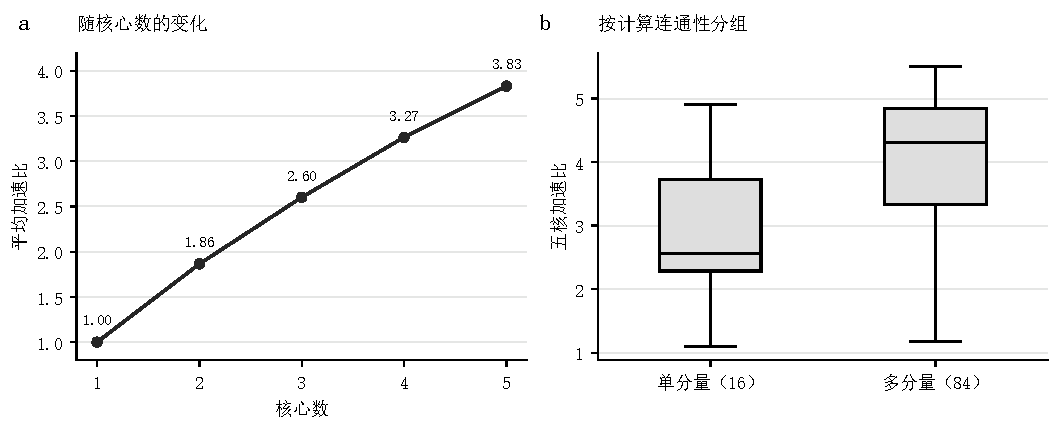
\includegraphics[width=\linewidth]{figures/fig6_1.pdf}
\caption{问题一的加速比结果。左图为每种核数下 100 图的算术平均，单核值按定义为 1；右图为五核下按弱连通分量数分组的分布。箱体表示四分位区间，中线为中位数，须延至 1.5 倍四分位距内的最远观测，点为其外观测。}
\label{fig:q1-result}
\end{figure}

五核平均加速比为 3.8311。多分量图的五核平均值为 4.0041，单分量图为 2.9228，表明输入结构对可利用的并行性有明显影响。多分量允许在较少新增依赖的条件下分配负载；单分量则通常需要在并行化与边界代价之间作出取舍。这一差异与独立分量提供可直接分配计算块的机制一致，分组内仍存在较大离散，故还需观察逐图对照。

与仅采用完整分量装箱的同批五核方案相比，增加结构切分与有限调度调整后，38 个图耗时下降、2 个图上升、60 个图不变。改进集中在完整分量分配以外的候选被选中后取得收益的输入上，少数退步反映了代理排序与实际执行的差异。五核平均额外搬运中，缓存换入换出占 7.423 MiB；任务边界之外的核内空间开销已达到不可忽略的规模。场景 B 延长了同核张量的可驻留范围，对这部分开销需要进一步建模。

\begin{figure}[htbp]
\centering
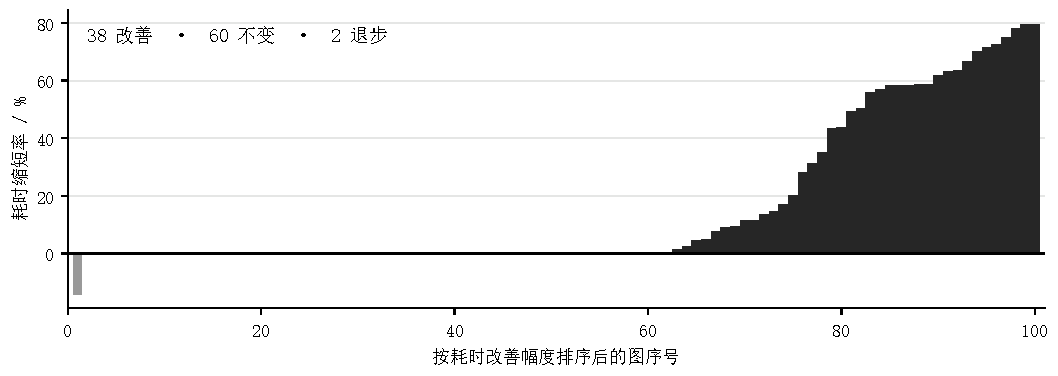
\includegraphics[width=\linewidth]{figures/fig6_2.pdf}
\caption{五核下相对于完整分量装箱的逐图耗时变化。横轴为全部 100 图按改善幅度排序后的序号，纵轴为 $100(1-T_A/T_{\rm component})$；零线以上表示扩展结构候选后的最终方案更快。该对照在同一场景 A 下验收，用于观察候选扩展及选择的综合作用。}
\label{fig:q1-comparator}
\end{figure}

图~\ref{fig:q1-comparator} 保留全部未改善和退步的用例。大量零变化说明在这些图上，低边界代价的分量分配已经足以被最终规则保留；正向尾部反映了内部切分和任务顺序调整的价值。两个退步用例则提示，有限候选中的代理最优仍可能低于分量对照的实际表现，继续增加构造数量并不能自动修复这一排序误差。
